% \documentclass[
%    tikz,
%    %border=1pt
% ]{standalone}

\documentclass{article}

\usepackage{verbatim}
\usepackage{amssymb}
\usepackage{amsmath}

\usepackage{tikz}

%\usepackage{tikz-cd}
\usepackage{pgfplots}
\usepackage[utf8]{inputenc}
\usepackage[upright]{fourier}
\usetikzlibrary{arrows,automata,positioning,matrix,cd,babel,matrix,arrows,decorations.pathmorphing,intersections}
\usetikzlibrary{intersections}

\usepackage[many]{tcolorbox}

\usepackage{graphicx,subcaption}




\pgfplotsset{compat=1.12}

\usepackage{tikz}
\usetikzlibrary{arrows,positioning,calc}
\usepackage{tikz}
\usepackage{cancel}
\usepackage{color}
\usetikzlibrary{shapes.geometric, arrows}



 % Enables pgfplots to reset the color cycle within a plot via \pgfplotsset{cycle list set=0}
% Credit to Jake in thread http://tex.stackexchange.com/questions/74315/command-to-set-cycle-list-position

\makeatletter
\def\pgfplots@getautoplotspec into#1{%
    \begingroup
    \let#1=\pgfutil@empty
    \pgfkeysgetvalue{/pgfplots/cycle multi list/@dim}\pgfplots@cycle@dim
    %
    \let\pgfplots@listindex=\pgfplots@numplots
    %%% Start new code
    \pgfkeysgetvalue{/pgfplots/cycle list set}\pgfplots@listindex@set
    \ifx\pgfplots@listindex@set\pgfutil@empty
    \else 
        \c@pgf@counta=\pgfplots@listindex
        \c@pgf@countb=\pgfplots@listindex@set
        \advance\c@pgf@countb by -\c@pgf@counta
        \globaldefs=1\relax
        \edef\setshift{%
            \noexpand\pgfkeys{
                /pgfplots/cycle list shift=\the\c@pgf@countb,
                /pgfplots/cycle list set=
            }
        }%
        \setshift%
    \fi
    %%% End new code    
    \pgfkeysgetvalue{/pgfplots/cycle list shift}\pgfplots@listindex@shift
    \ifx\pgfplots@listindex@shift\pgfutil@empty
    \else
        \c@pgf@counta=\pgfplots@listindex\relax
        \advance\c@pgf@counta by\pgfplots@listindex@shift\relax
        \ifnum\c@pgf@counta<0
            \c@pgf@counta=-\c@pgf@counta
        \fi
        \edef\pgfplots@listindex{\the\c@pgf@counta}%
    \fi
    \ifnum\pgfplots@cycle@dim>0
        % use the 'cycle multi list' feature.
        %
        % it employs a scalar -> multiindex map like
        % void fromScalar( size_t d, size_t scalar, size_t* Iout, const size_t* N )
        % {
        %   size_t ret=scalar;
        %   for( int i = d-1; i>=0; --i ) {
        %       Iout[i] = ret % N[i];
        %       ret /= N[i];
        %   }
        % }
        % to get the different indices into the cycle lists.
        %-------------------------------------------------- 
        \c@pgf@counta=\pgfplots@cycle@dim\relax
        \c@pgf@countb=\pgfplots@listindex\relax
        \advance\c@pgf@counta by-1
        \pgfplotsloop{%
            \ifnum\c@pgf@counta<0
                \pgfplotsloopcontinuefalse
            \else
                \pgfplotsloopcontinuetrue
            \fi
        }{%
            \pgfkeysgetvalue{/pgfplots/cycle multi list/@N\the\c@pgf@counta}\pgfplots@cycle@N
            % compute list index:
            \pgfplotsmathmodint{\c@pgf@countb}{\pgfplots@cycle@N}%
            \divide\c@pgf@countb by \pgfplots@cycle@N\relax
            %
            \expandafter\pgfplots@getautoplotspec@
                \csname pgfp@cyclist@/pgfplots/cycle multi list/@list\the\c@pgf@counta @\endcsname
                {\pgfplots@cycle@N}%
                {\pgfmathresult}%
            \t@pgfplots@toka=\expandafter{#1,}%
            \t@pgfplots@tokb=\expandafter{\pgfplotsretval}%
            \edef#1{\the\t@pgfplots@toka\the\t@pgfplots@tokb}%
            \advance\c@pgf@counta by-1
        }%
    \else
        % normal cycle list:
        \pgfplotslistsize\autoplotspeclist\to\c@pgf@countd
        \pgfplots@getautoplotspec@{\autoplotspeclist}{\c@pgf@countd}{\pgfplots@listindex}%
        \let#1=\pgfplotsretval
    \fi
    \pgfmath@smuggleone#1%
    \endgroup
}

\pgfplotsset{
    cycle list set/.initial=
}
\makeatother


\pgfplotsset{
    every axis plot post/.style={
        line join=round
    },
    every axis/.append style={font=\large},
    every tick label/.append style={font=\large}
}

\pgfplotsset{yticklabel style={text width=1.5em,align=right}}


\usepackage{pgfplotstable}
\usepackage{booktabs}

\begin{document}

\thispagestyle{empty}
%%%%%%%%%%%%%%%%%%%%%%%%%%%%%%%%%%%%%%%%%%%%%%%%%%%%%%%%%%%%%%%%%%%%%%%%%%%%%%%%%%%%%%%%%%%%%%%%%%%%%%%%%%%%%%%%%%%%%%%%%%%%%%%%%%%%%%%%%%%%%%%
%%%%%%%%%%%%%%%%%%%%%%%%%%%%%%%%%%%%%%%%%%%%% FIGURE 2 %%%%%%%%%%%%%%%%%%%%%%%%%%%%%%%%%%%%%%%%%%%%%%%%%%%%%%%%%%%%%%%%%%%%%%%%%%%%%%%%%%%%%%%%
%%%%%%%%%%%%%%%%%%%%%%%%%%%%%%%%%%%%%%%%%%%%%%%%%%%%%%%%%%%%%%%%%%%%%%%%%%%%%%%%%%%%%%%%%%%%%%%%%%%%%%%%%%%%%%%%%%%%%%%%%%%%%%%%%%%%%%%%%%%%%%%


\begin{figure}


 
% % %%%%%%%%%%%%%%%%%%%%%%%%%%%%%%%%%%%%%%%%%%%%%%%%%%%%%%%%%%%%%%%%%%%%%%%%%%%%%%%%%%%%%%%%%%%%%%%%%%%%%%%%%%%%%%%%%%%%%%%%%%%%%%%%%%%%%%%%%%%
% %     %%%%%%%%%%%%%%%%%%%%%%%%%%%%%%%%%%%%%%%%%%%%% PART A %%%%%%%%%%%%%%%%%%%%%%%%%%%%%%%%%%%%%%%%%%%%%%%%%%%%%%%%%%%%%%%%%%%%%%%%%%%%%%%%%%
% %     %%%%%%%%%%%%%%%%%%%%%%%%%%%%%%%%%%%%%%%%%%%%%%%%%%%%%%%%%%%%%%%%%%%%%%%%%%%%%%%%%%%%%%%%%%%%%%%%%%%%%%%%%%%%%%%%%%%%%%%%%%%%%%%%%%%%%%%%%%%
\vspace{0.2cm}
\hspace{-2.5cm}

\hspace{-2.5cm}

\begin{tikzpicture}[every plot/.append style={very thick}]
	% Part A
	\node[draw=none, fill=none] at (2.2,3.5) {\Large A};
	\node[circle, draw=black, fill=none] at (4,2) (plus){\large $A$};
	\node[circle, draw=black, fill=none] at (4,0) (minus){\large $B$};
	% \draw [transform canvas={xshift=-2.5pt}](minus) -- (plus);
	% \draw [transform canvas={xshift=2.5pt}](minus) -- (plus);
	\draw	(minus)to[out=60,in=-60] (plus);
	\draw	(minus)to[out=130,in=-130] (plus);
%	\draw	(minus)to[out=20,in=70] (plus);
	\filldraw (4.23,1.63) circle (3pt);
	\filldraw (3.77,0.37) circle (3pt);
	\node[draw=none, fill=none] at (2.6,1) (E){\large E$_{ext}$};

	\draw	(E)to[out=0,in=180] (minus);
	\draw	(E)to[out=0,in=180] (plus);
	
	% Part B
	\node[draw=none, fill=none] at (5.5,3.5) {\Large B};
	\node[draw=none, fill=none, anchor=north west] at (6,3.5) (rasterplot) {
		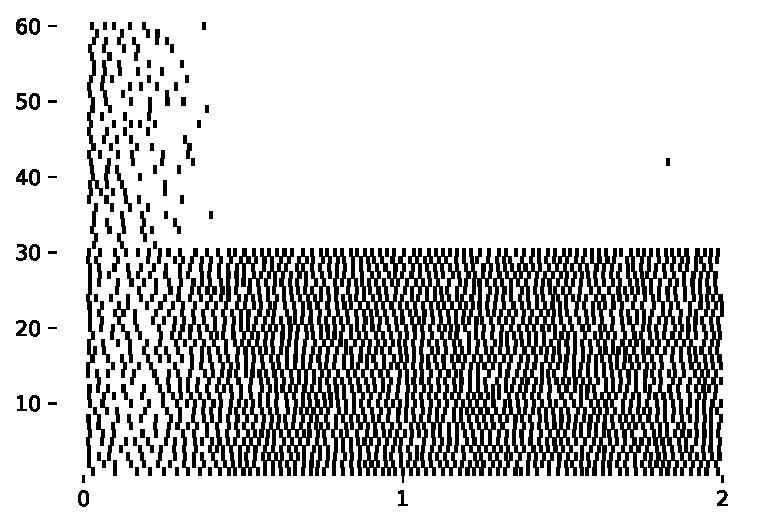
\includegraphics[width=220pt]{raster_decision}
	};
	\node[draw=none, fill=none] at (11,-1.7) {$t$ (sec)};
	\node[draw=none, fill=none, rotate=90, anchor=south] at (5.8,1) {Neuron};
	\node[draw=none, fill=none, rotate=90, anchor=south] at (6.2,2) {\small pop. A};
	\node[draw=none, fill=none, rotate=90, anchor=south] at (6.2,0) {\small pop. B};
	
	% Part C
	\node[draw=none, fill=none] at (2.2,-2) {\Large C};
	\node[draw=none, fill=none] at (4.2,-8) {
		\begin{axis}
       [
         name=figB,
         axis line style = { draw = none },
         width=340pt,
         height=220pt,
         xtick           = {0, 1000, 2000}         ,
         xticklabels     = {0, 1, 2} ,
         ytick           = {1, 2, 3}         ,
         tick pos        = left           ,
         xlabel={$t$ (sec)},
         ylabel = {Fluorescence},
       ]


	\addplot [ultra thick, no markers, black] table [x index=0, y index=1, col sep=comma, mark=circle]{CSV/figure_4_5_calc_nonoise0.csv};
	\addplot [only marks, black, mark=diamond*, mark size=1.5pt] table [x index=0, y index=1, col sep=comma]{CSV/figure_4_5_calc_sample0.csv};

	\addplot [ultra thin, no markers, gray] table [x index=0, y index=1, col sep=comma, mark=circle]{CSV/figure_4_5_calc_nonoise1.csv};
	\addplot [only marks, gray, mark=diamond*, mark size=1.5pt] table [x index=0, y index=1, col sep=comma]{CSV/figure_4_5_calc_sample1.csv};

	%\addplot [no markers, thin, gray, dashed] coordinates {(1.5,1.0) (2.5,1.0)};
\end{axis}

	};
	
	% Part C inset
	\node[draw=none, fill=none] at (10.4,-5.4) {
		\begin{axis}
       [
         name=figB,
         axis line style = { draw = none },
         width=120pt,
         height=80pt,
         xtick           = {0, 500, 1000}         ,
         xticklabels     = {0, 0.5, 1} ,
         ytick           = {0, 0.2}         ,
         tick pos        = left           ,
         xlabel={$t-t_{\textrm{spike}}$} ,
         ylabel = {$\Delta F/F$},
       ]


		%\addplot [no markers, black] table [x index=0, y index=1, col sep=comma, mark=circle]{CSV/figure3_panel2_line1.csv};

		\addplot [no markers, black] table [x index=0, y index=1, col sep=comma, mark=circle]{CSV/figure_4_5_fred_inset.csv};

		%\addplot [no markers, thin, gray, dashed] coordinates {(1.5,1.0) (2.5,1.0)};
	\end{axis}

	};


\end{tikzpicture}

%\begin{tikzpicture}[every plot/.append style={very thick}]
%\node[draw=none, fill=none] at (-1,4.8) {\Large C};
%\node[draw=none, fill=none] at (2.85,4.8) {\large $E_{ext}=2.5$ nS};
%%\node[draw=none, fill=none] at (2.05,3.4) {\large $\sigma=0.2$};
%\begin{axis}
%       [
%         axis line style = { draw = none },
%         width=0.6\linewidth,
%         height=0.5\linewidth,
%         xtick           = {0, 3}         ,
%         ytick           = {0, 3}         ,
%         tick pos        = left           ,
%         xlabel={$-$ pop. output (nS)},
%         ylabel = {$+$  pop. output (nS)},
%         xmin=-0.2,xmax=3.8,
%         ymin=-0.2,ymax=3.8
%       ]
%
%
%\addplot [
%quiver={u=\thisrowno{2},v=\thisrowno{3}, scale arrows=0.5}, 
%gray, ->, >=stealth, mark options={scale=0.2}
%] table [x index=0, y index=1, col sep=comma, mark=circle]{CSV/figure3_panel1_line1_ind12.csv};
%
%\addplot [no markers, black, thick, dashed] table [x index=0, y index=1, col sep=comma, mark=circle]{CSV/figure3_panel1_line2_ind12.csv};
%
%\addplot [no markers, black, thick, dotted] table [x index=0, y index=1, col sep=comma, mark=circle]{CSV/figure3_panel1_line3_ind12.csv};
%
%\addplot [
%    point meta=explicit,
%    scatter, only marks,
%    visualization depends on=\thisrowno{4}\as\metacolorind,
%    scatter/@pre marker code/.code={
%        \pgfplotsset{%
%        mark size=(1+0.003*\pgfplotspointmetatransformed)},%
%        \ifdim\metacolorind pt<1.0pt
%            \def\markopts{color=red}%
%        \else
%            \def\markopts{color=blue}%
%        \fi
%        \expandafter\scope\expandafter[\markopts]
%    },%
%    scatter/@post marker code/.code={%
%        \endscope
%    },%
%    ] table [x index=0, y index=1, meta index=2, col sep=comma]{CSV/figure3_panel1_line4_ind12.csv};
%
%
%\end{axis}
%
%\end{tikzpicture}
%% % %%%%%%%%%%%%%%%%%%%%%%%%%%%%%%%%%%%%%%%%%%%%%%%%%%%%%%%%%%%%%%%%%%%%%%%%%%%%%%%%%%%%%%%%%%%%%%%%%%%%%%%%%%%%%%%%%%%%%%%%%%%%%%%%%%%%%%%%%%%
%% %     %%%%%%%%%%%%%%%%%%%%%%%%%%%%%%%%%%%%%%%%%%%%% FIGURE 2 D %%%%%%%%%%%%%%%%%%%%%%%%%%%%%%%%%%%%%%%%%%%%%%%%%%%%%%%%%%%%%%%%%%%%%%%%%%%%%%%%%%
%% %     %%%%%%%%%%%%%%%%%%%%%%%%%%%%%%%%%%%%%%%%%%%%%%%%%%%%%%%%%%%%%%%%%%%%%%%%%%%%%%%%%%%%%%%%%%%%%%%%%%%%%%%%%%%%%%%%%%%%%%%%%%%%%%%%%%%%%%%%%%%
%\hspace{0.5cm}
%\begin{tikzpicture}[every plot/.append style={very thick}]
%\node[draw=none, fill=none] at (-1,4.8) {\Large D};
%\begin{axis}
%       [
%         name=figB,
%         axis line style = { draw = none },
%         width=0.6\linewidth,
%         height=0.5\linewidth,
%         xtick           = {1.5,2,2.5}         ,
%         ytick           = {0, 0.5, 1, 1.5}         ,
%         tick pos        = left           ,
%         xlabel={$E_{ext}$ (nS)},
%         ylabel = {Eigenvalues},
%       ]
%
%
%\addplot [no markers, black] table [x index=0, y index=1, col sep=comma, mark=circle]{CSV/figure3_panel2_line1.csv};
%
%\addplot [no markers, black] table [x index=0, y index=2, col sep=comma, mark=circle]{CSV/figure3_panel2_line1.csv};
%
%\addplot [no markers, thin, gray, dashed] coordinates {(1.5,1.0) (2.5,1.0)};
%
%
%\end{axis}
%
%% Manually tikz-picture arrows
%\draw [->, >=latex, very thick] (5,2.0) -- (5.65,1.35);
%\node [draw=none,fill=none] at (4.6, 1.6) {Unstable};
%\draw [->, >=latex, very thick] (5,2.0) -- (5.65,2.65);
%\node [draw=none,fill=none] at (4.6, 2.4) {Stable};
%


\end{figure}

\end{document}

